\documentclass{newsiambook}

\usepackage{hyperref}
\usepackage{import}
\usepackage{amsmath, amsfonts, amscd, amssymb}
\usepackage{mathtools}
\usepackage{epsfig}
\usepackage{graphicx}
\usepackage{url}
\usepackage{mathrsfs}
\usepackage{makeidx}
\usepackage{multicol}
\usepackage{color}
\usepackage{crop}
\usepackage{verbatim}
\usepackage{listings}
\usepackage{pseudocode}
\usepackage{framed}

%------------------------------------------------------------------------------%
% command.tex                                                                  %
% This file contains the various environments and other misc. commands         %
%------------------------------------------------------------------------------%

%BibTeX project-wide style
\bibliographystyle{alpha}

%counter for problems. reset each chapter
\newcounter{problemnum}[chapter]
\newtheoremup{problemnum}{Problem}

\newcommand{\objective}[1]{{\bf Lab Objective: } \emph{#1} \bigskip}
\renewcommand{\chaptername}{Lab}
\renewcommand{\bibname}{References}

\newcommand{\lab}[3]{\chapter[#3]{#1: #2}}

% Various commands that make life easier
\newcommand{\argmax}{\mbox{argmax}}
\newcommand{\indicator}[1]{\mathbbm{1}_{\left[#1\right] }}
\providecommand{\abs}[1]{\left\lvert#1\right\rvert}
\providecommand{\norm}[1]{\left\lVert#1\right\rVert}
\providecommand{\set}[1]{\lbrace#1\rbrace}
\providecommand{\setconstruct}[2]{\lbrace#1:#2\rbrace}
\providecommand{\res}[1]{\underset{#1}{Res}}           % Residue
\providecommand{\Res}[1]{\underset{#1}{Res}}           % Residue

\newcommand{\li}[1]{\lstinline[prebreak=]!#1!}

\newcommand{\ipt}[2]{\langle #1,#2 \rangle}
\newcommand{\ip}{\int_{-\infty}^{+\infty}}

\renewcommand{\ker}[1]{\mathcal{N}(#1)}
\newcommand{\ran}[1]{\mathcal{R}(#1)}

% Full line comments in the Algorithmic environment.
\algnewcommand{\LineComment}[1]{\State \(\triangleright\) #1}

\newenvironment{amatrix}[1]{%
\left(\begin{array}{@{}*{#1}{c}|c@{}}
}{%
\end{array}\right)
}

\newenvironment{dmatrix}[2]{%
\left(\begin{array}{@{}*{#1}{c}|*{#2}{c}@{}}
}{%
\end{array}\right)
}


%%Frame environments
\definecolor{shadecolor}{gray}{0.90}
\mdfdefinestyle{problem}{backgroundcolor=shadecolor,
                         hidealllines=true,
                         skipabove=10pt,
                         skipbelow=10pt,
                         innertopmargin=15pt,
                         innerbottommargin=15pt,
                         innerleftmargin=15pt,
                         innerrightmargin=15pt}

\definecolor{warning}{RGB}{255,231,231}
\definecolor{warnline}{RGB}{255,15, 15}
\newmdenv[
  roundcorner=10pt,
  skipabove=10pt
  skipbelow=10pt
  leftmargin=20pt,
  rightmargin=20pt,
  backgroundcolor=warning,
  innertopmargin=10pt,
  innerbottommargin=10pt,
  innerleftmargin=10pt,
  middlelinewidth=0pt,
  everyline=true,
  linecolor=warnline,
  linewidth=1pt,
  font=\normalfont\normalsize,
  frametitlefont=\large\bfseries,
  frametitleaboveskip=1em,
  frametitlerule=true,
  frametitle={\sc Warning}
]{warn}

\definecolor{information}{RGB}{231,231,255}
\definecolor{infoline}{RGB}{15,15, 255}
\newmdenv[
  roundcorner=10pt,
  skipabove=10pt
  skipbelow=10pt
  leftmargin=20pt,
  rightmargin=20pt,
  backgroundcolor=information,
  innertopmargin=10pt,
  innerbottommargin=10pt,
  innerleftmargin=10pt,
  middlelinewidth=0pt,
  everyline=true,
  linecolor=infoline,
  linewidth=1pt,
  font=\normalfont\normalsize,
  frametitlefont=\large\bfseries,
  frametitleaboveskip=1em,
  frametitlerule=true,
  frametitle={\sc Note}
]{info}

\newenvironment{problem}{\begin{mdframed}[style=problem]\begin{problemnum}}{\end{problemnum}\end{mdframed}}


\newenvironment{amatrix}[1]{%
\left(\begin{array}{@{}*{#1}{c}|c@{}}
}{%
\end{array}\right)
}

\newenvironment{dmatrix}[2]{%
\left(\begin{array}{@{}*{#1}{c}|*{#2}{c}@{}}
}{%
\end{array}\right)
}

\newtheoremup{problemnum}{Problem}
\definecolor{shadecolor}{gray}{0.90}
\newenvironment{problem}{\begin{shaded}\begin{problemnum}}{\end{problemnum}\end{shaded}}

\newcommand{\ipt}[2]{\langle #1,#2 \rangle}
\newcommand{\ip}{\int_{-\infty}^{+\infty}}

\renewcommand{\ker}[1]{\mathcal{N}(#1)}
\newcommand{\ran}[1]{\mathcal{R}(#1)}

\def\0{{\bf 0}}
\def\a{{\bf a}}
\def\b{{\bf b}}
\def\e{{\bf e}}
\def\p{{\bf p}}
\def\q{{\bf q}}
\def\u{{\bf u}}
\def\v{{\bf v}}
\def\w{{\bf w}}
\def\x{{\bf x}}
\def\y{{\bf y}}
\def\z{{\bf z}}
\def\subspace{\lhd}

\def\CalL{\mathcal{L}}
\def\CalO{\mathcal{O}}
\def\CalV{\mathcal{V}}
\def\CalU{\mathcal{U}}
\def\bU{{\bar{u}}}
\def\R{\Re e}
\def\I{\Im m}
\def\M{M_n}

\renewcommand{\labelenumi}{\textnormal{(\alph{enumi}).}}

% \lstset{basicstyle=\footnotesize\ttfamily,
%         keywordstyle=\color{blue}\bfseries,
%         tabsize=4,
%         frame=tb,
%         captionpos=b,
%         title=\lstname,
%         abovecaptionskip=-5pt,
%         belowcaptionskip=-5pt,
%         breaklines=true,
%         breakatwhitespace=false,
%         showstringspaces=false}

\lstset{basicstyle=\footnotesize\ttfamily,
		keywordstyle=\color{blue}\bfseries\ttfamily,
		tabsize=4,
		frame=tb,
		captionpos=b,
		breaklines=true,
		breakatwhitespace=false,
		title=\lstname,
		showstringspaces=false}


\lstdefinestyle{fromfile}{frame=single,
			  numbers=left,
			  numberstyle=\tiny,
			  stepnumber=2,
			  numbersep=7pt,
			  numberfirstline=true}

%----PYTHON STYLES----                          
\lstdefinestyle{python}{language=Python}
\lstdefinestyle{pythonnums}{language=Python,
                            numbers=left,
                            numberstyle=\tiny,
                            stepnumber=2,
                            numbersep=7pt,
                            numberfirstline=true}

%----MATLAB STYLES----
\lstdefinestyle{matlab}{language=Matlab}
\lstdefinestyle{matlabnums}{language=Matlab,
                            numbers=left,
                            numberstyle=\tiny,
                            stepnumber=2,
                            numbersep=7pt,
                            numberfirstline=true}




\crop
\makeindex

%\includeonly{./Applications_Combined/PageRank}
%\includeonly{./Algorithms_PyLabs/Complexity_py}

\DeclareMathOperator{\res}{res}           % Residue
\DeclareMathOperator{\Res}{Res}           % Residue

\begin{document}

%-------------------------------------------------------------

  \newcommand{\li}[1]{\lstinline[style=python]!#1!}

\newenvironment{pseudo}[2]
    {\begin{pseudocode}[shadowbox]{#1}{#2}}
    {\end{pseudocode}}

%----------------------------------------------------------------
%Book cover and Front matter
\thispagestyle{empty}
\begin{center}
{\Huge \bf Applied Mathematics and Computing}

\vspace{10mm}
\vspace{20mm}

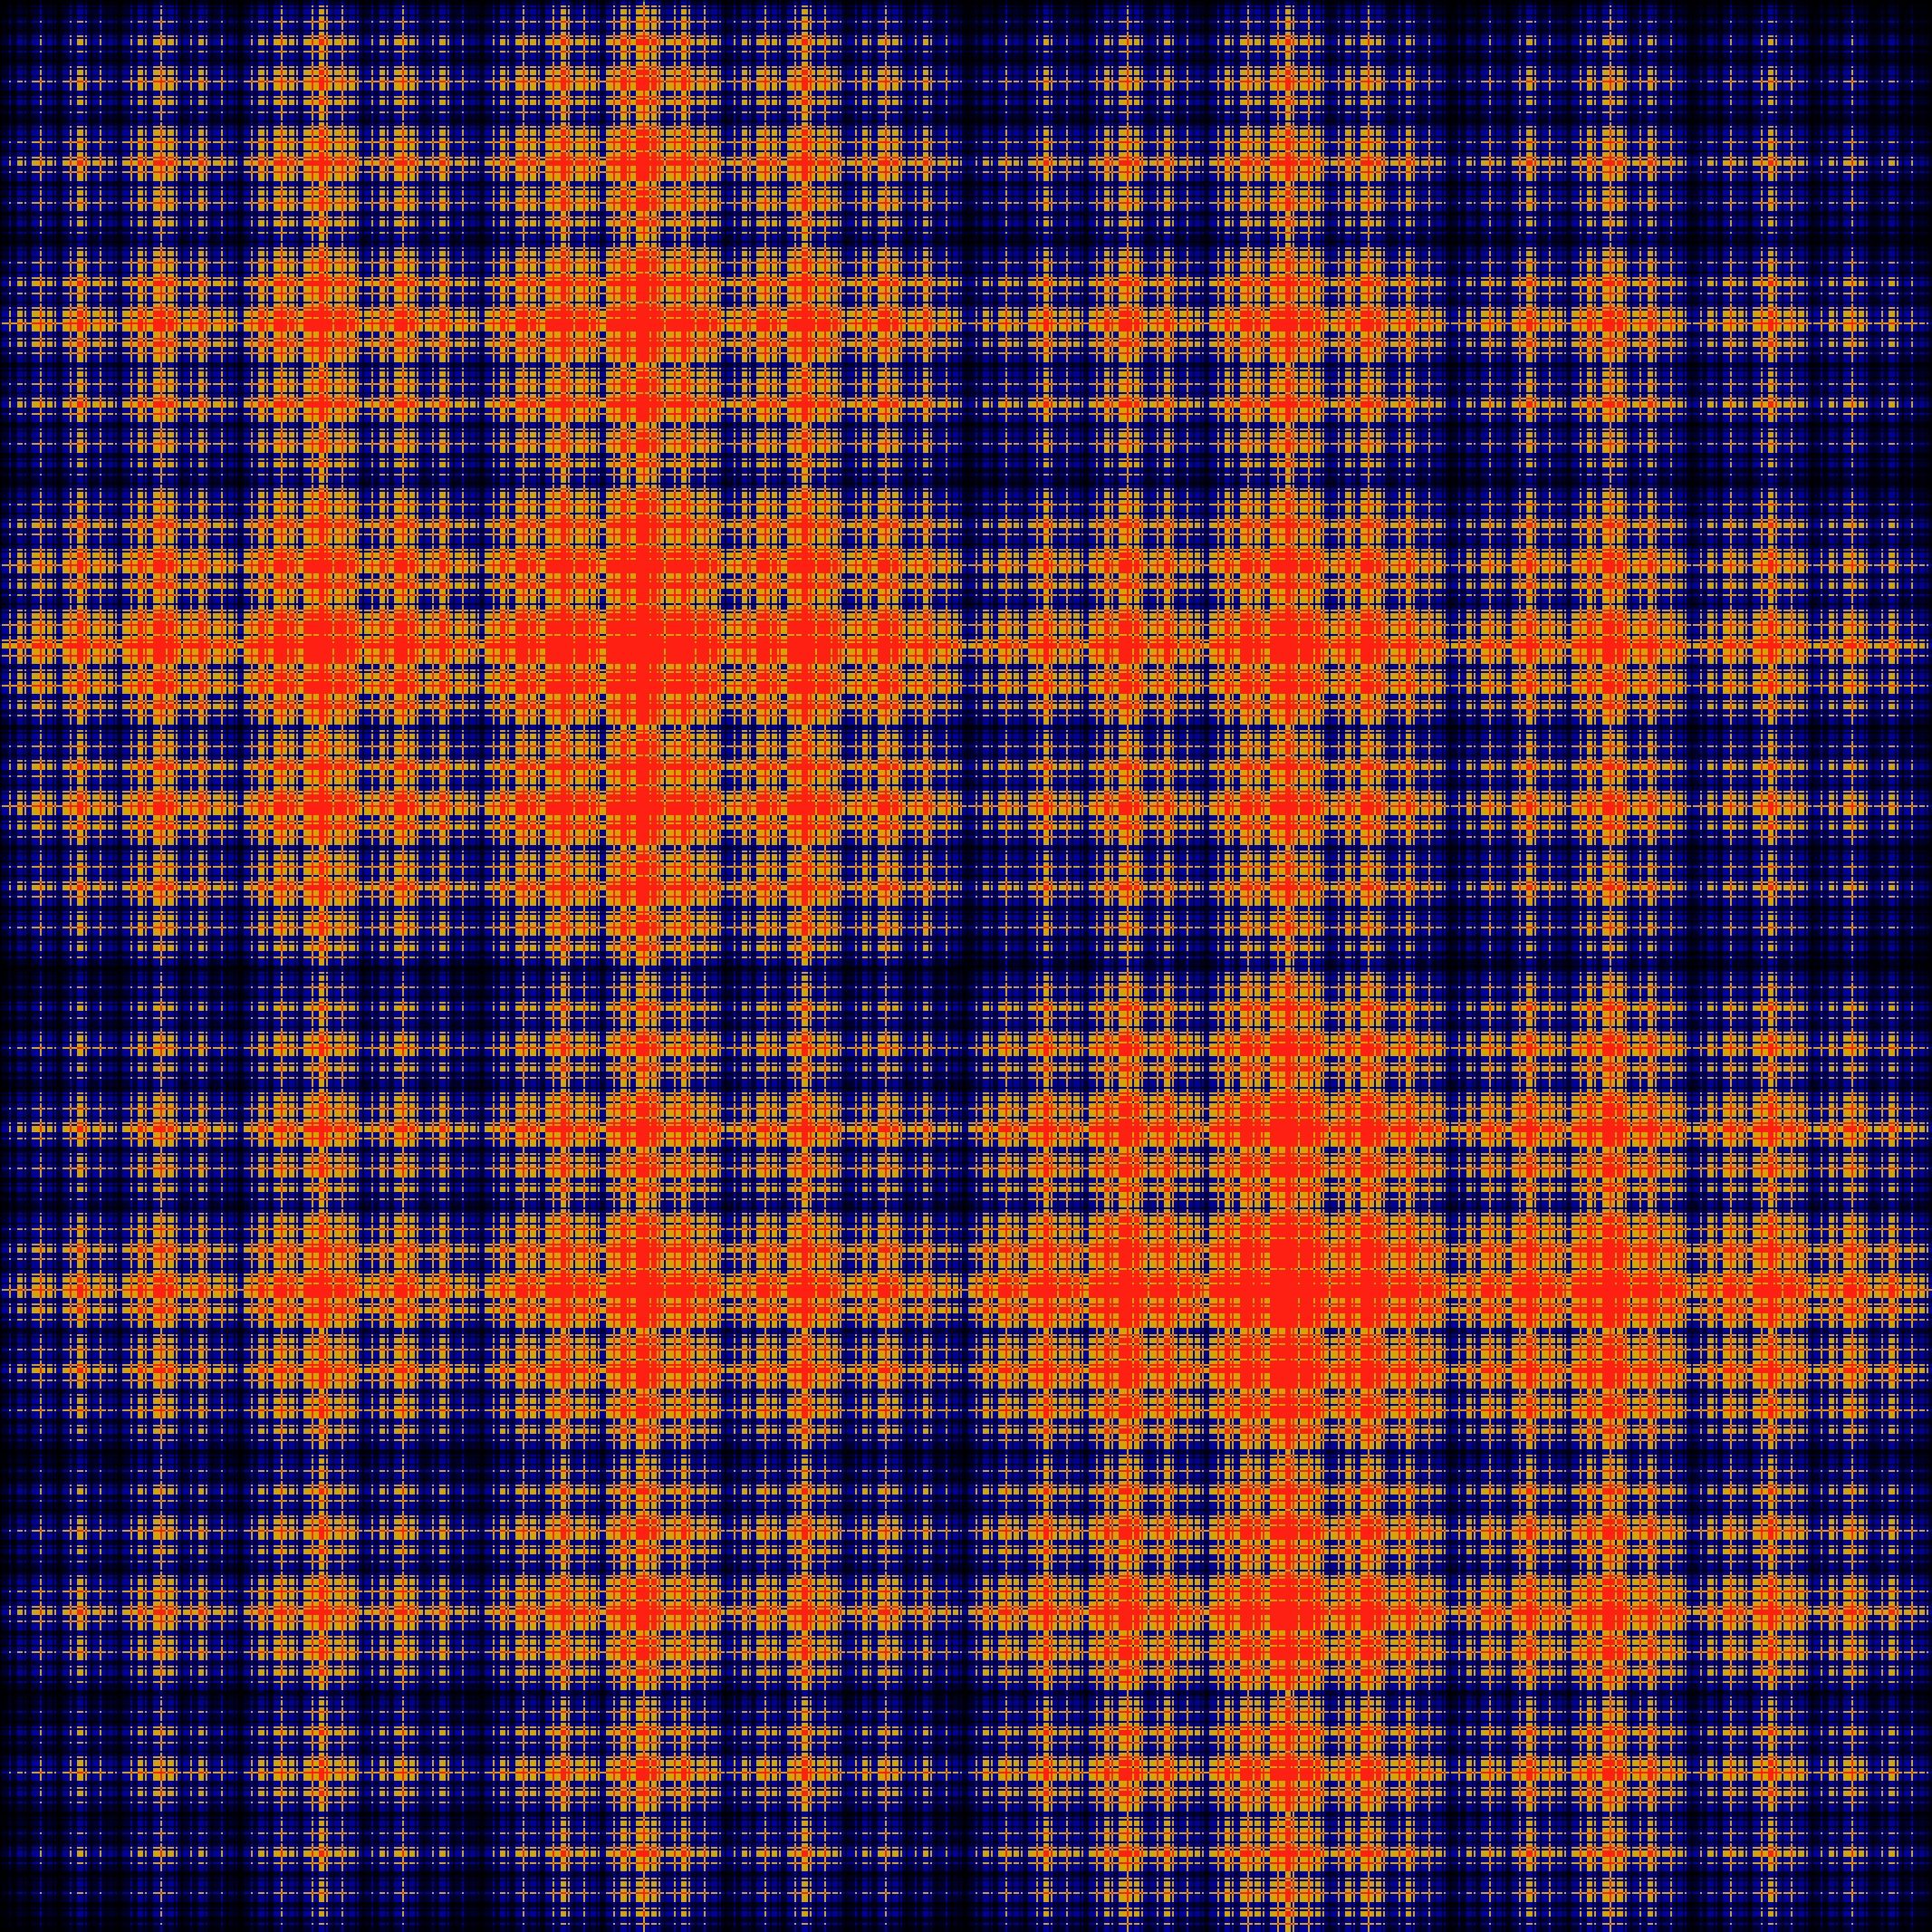
\includegraphics[scale = .25]{Cover}
\end{center}
\frontmatter
\begin{contributors}
\contributor{J.~Humpherys}{Brigham Young University}
\contributor{J.~Webb}{Brigham Young University}
\contributor{R.~Murray}{Brigham Young University}
\contributor{J.~West}{University of Michigan}
\contributor{R.~Grout}{Brigham Young University}
\contributor{K.~Finlinson}{Brigham Young University}
\end{contributors}

%------------------------------------------------------------------
%The preface, which will presumably be longer in the future

\begin{thepreface}
This lab manual is designed to accompany the textbook \emph{Foundations of Applied Mathematics} by Dr.~J.~Humpherys.

\vfill
\copyright{This work is licensed under the Creative Commons Attribution 3.0 United States 
License.  You may copy, distribute, and display this copyrighted work only if you give 
credit to Dr.~J.~Humpherys. All derivative works must include an attribution to Dr.~J.~Humpherys as the owner of this work as well as the web address to 
\\\centerline{\url{https://github.com/ayr0/numerical_computing}}\\ as the original source of 
this 
work.\\To view a copy of the Creative Commons Attribution 3.0 License, 
visit\\\centerline{\url{http://creativecommons.org/licenses/by/3.0/us/}} or send a letter to 
Creative Commons, 171 Second Street, Suite 300, San Francisco, California, 94105, USA.}

\vfill
\centering
\includegraphics[height=1.2cm]{by}
\vfill
\end{thepreface}
%-----------------------------------------------------------------

\setcounter{tocdepth}{1}
\tableofcontents

\mainmatter


\part{Linear Transforms}
%\subimport{Ch0_Py/}{Py0}
\subimport{./Algorithms/Matrices/}{Matrices1}
\subimport{./Algorithms/Matrices/}{Matrices2}
\subimport{./Applications/MarkovGraph/}{MarkovGraph_C}
\subimport{./Algorithms/ElemMatrices/}{ElemMatr_C}
\subimport{./Applications/Leontief/}{Leontief_C}

\part{Inner Product Spaces}
%Correlation and Covariance
\subimport{./Algorithms/QR/}{QR_C}
\subimport{./Algorithms/Householder/}{Householder}
\subimport{./Applications/Statistics/}{Stats1_C}


\part{Spectral Theory}
\subimport{./Algorithms/EigSolver/}{Eig_C}
\subimport{./Algorithms/Cholesky/}{Cholesky_C}
\subimport{./Applications/SVD/}{SVD_C}

\part{Differentiation}
\subimport{./Algorithms/NumDeriv/}{FiniteDiff_C}
\subimport{./Applications/BeamBuckle/}{Beams_C}
\subimport{./Algorithms/MultiDeriv/}{FiniteDiff2_C}
\subimport{./Applications/ImgFilters/}{ImgFilters}

\part{Vector Spaces}
\subimport{./Applications/Matplotlib/}{matplotlib}


\part{Convex Analysis}

\part{Contractions}
\subimport{./Applications/NewtonsMethod/}{Newton_C}
\subimport{./Applications/Julia/}{Julia}
\subimport{./Algorithms/Broyden/}{Broyden}

\part{Riemann-Darboux Integration}
\subimport{./Algorithms/GaussQuad/}{GaussQuad}
\subimport{./Applications/MC/}{MC}

% \subimport{./Algorithms/Functions/}{Functions2}
% %\subimport{./Applications/Vectorization/}{Vectorization}
% 
% \subimport{./Applications/Recursion/}{Recursion}

\part{Curves and Surfaces}
\subimport{./Algorithms/Splines/}{Splines}
\subimport{./Applications/Tesselation/}{Tess}
\subimport{./Applications/NURBS/}{NURBS_C}

\part{Complex Integration}
\subimport{./Applications/ConfMaps/}{ConfMaps}
\subimport{./Applications/RiemannSphere/}{RiemannSphere_C}
\subimport{./Applications/ComplexIntegration/}{ComplexIntegration1}
\subimport{./Applications/ComplexIntegration/}{ComplexIntegration2}

\part{Spectral Calculus}
\subimport{./Algorithms/JordanSchur/}{Jordan}
\subimport{./Algorithms/Krylov/}{Krylov}
\subimport{./Applications/MarkovPerron/}{MarkovPerron}

\part{Generalized Inverses}
\subimport{./Algorithms/MoorePenrose/}{MP}
\subimport{./Algorithms/Drazin/}{Drazin}
\subimport{./Applications/MarkovCount/}{MarkovCount}

\part{Discrete Error Analysis}

\part{Permutations and Groups}



%\subimport{./Algorithms/Functions/}{Functions}

%-----------------------------------------------------------
%The next few labs are more programming tutorial labs, and are split by language
% \subimport{./Algorithms/Conditionals/}{Conditionals}
% \subimport{./Algorithms/Complexity/}{Complexity}

%-----------------------------------------------------------
%These labs are primarily Linear Algebra Labs (Factorizations and Applications)
%They are combined


%\subimport{./Algorithms/Givens/}{Givens} 
%\subimport{./Applications/OrthoPoly/}{OrthoPoly_C}

%\subimport{./Applications/EigGraph/}{EigGraph_C}


%------------------------------------------------------------
%These labs are more advanced programming labs. They are separated by language.

% \subimport{./Algorithms/Functions/}{Functions2}
% %\subimport{./Applications/Vectorization/}{Vectorization}
% 
% \subimport{./Applications/Recursion/}{Recursion}
% %We need a profiler lab here.


%\subimport{./Applications/NormsGeometry/}{Norms_Geometry}

%-----------------------------------------------------------
%These labs cover the basics of differentiation, Newton's method and a number of related applications. These are combined labs



%\subimport{./Applications/LevelSet/}{LevelSet}


%\subimport{./Applications/PageRank/}{PageRank}
%\subimport{./Algorithms/JacobiGaussSidel/}{Iterative1}
%\subimport{./Algorithms/SuccOverRelax/}{Iterative2}
%Need permission and web address for internet.dat



%\subimport{./Algorithms/Barycentric/}{Barycentric}

%\subimport{./Algorithms/NewtonCotes/}{NCInteg}
%\subimport{./Applications/VarianceReduction/}{VEGAS}



%\subimport{./Applications/ConfMaps/}{ConfMaps}

%\subimport{./Algorithms/PerspectiveTransform/}{PerspTrans_C}
%\subimport{./Applications/RiemannSphere/}{RiemannSphere_C}

%----------------------------------------------------------------
%These labs cover a wide variety of applications, and finish off the book. They will be combined

%\subimport{./Applications/RayTracing/}{RayTracing}

%\subimport{./Applications/LagSylvInterp/}{LagSylvInterp}
%\subimport{./Applications/MoorePenrose/}{MPApp}

\end{document}
